一维势箱模型是共轭分子的一个粗糙近似,在这个模型中,假设$\pi$电子在共轭的碳骨架中自由运动,因此这个模型也被称为自由电子模型(FEM )。势箱的长度可以通过$L=n_C\times1.40\mathrm{\AA}$估计,其中$L$是势箱长度,$n_C$是碳的个数。此外,在电子填入能级时,泡利不相容原理是适用的,一维势箱的能量公式如下:

$$
E_n=\frac{n^2L^2}{8mL^2}
$$

\noindent 其中$m$是粒子质量,$h$是普朗克常量,$n$是正整数。

对1,3,5,7-辛四烯分子使用FEM:

\noindent\textbf{18.1.} 画出能级图,填入电子,并计算轨道能量。

\noindent\textbf{18.2.} 计算分子的总$\pi$电子能量。

\noindent\textbf{18.3.}
确定可将电子从最高占有轨道(HOMO)激发到最低未占有轨道(LUMO)的光的波长(结果用nm表示)。

对于二维共轭体系,我们会使用二维势箱模型,在这种情况下,能量公式如下:

$$
E_{n_1,n_2}=\frac{h^2}{8m}\left(\frac{n^2_1}{L_1^2}+\frac{n^2_2}{L_2^2}\right)
$$

\noindent 其中$L_1$和$L_2$是长度,$n_1$和$n_2$分别是两个维度的量子数。

石墨烯是一种二维六边形晶格的碳原子片,其中每个顶点由一个原子构成。

\begin{figure}[h]
	\centering
	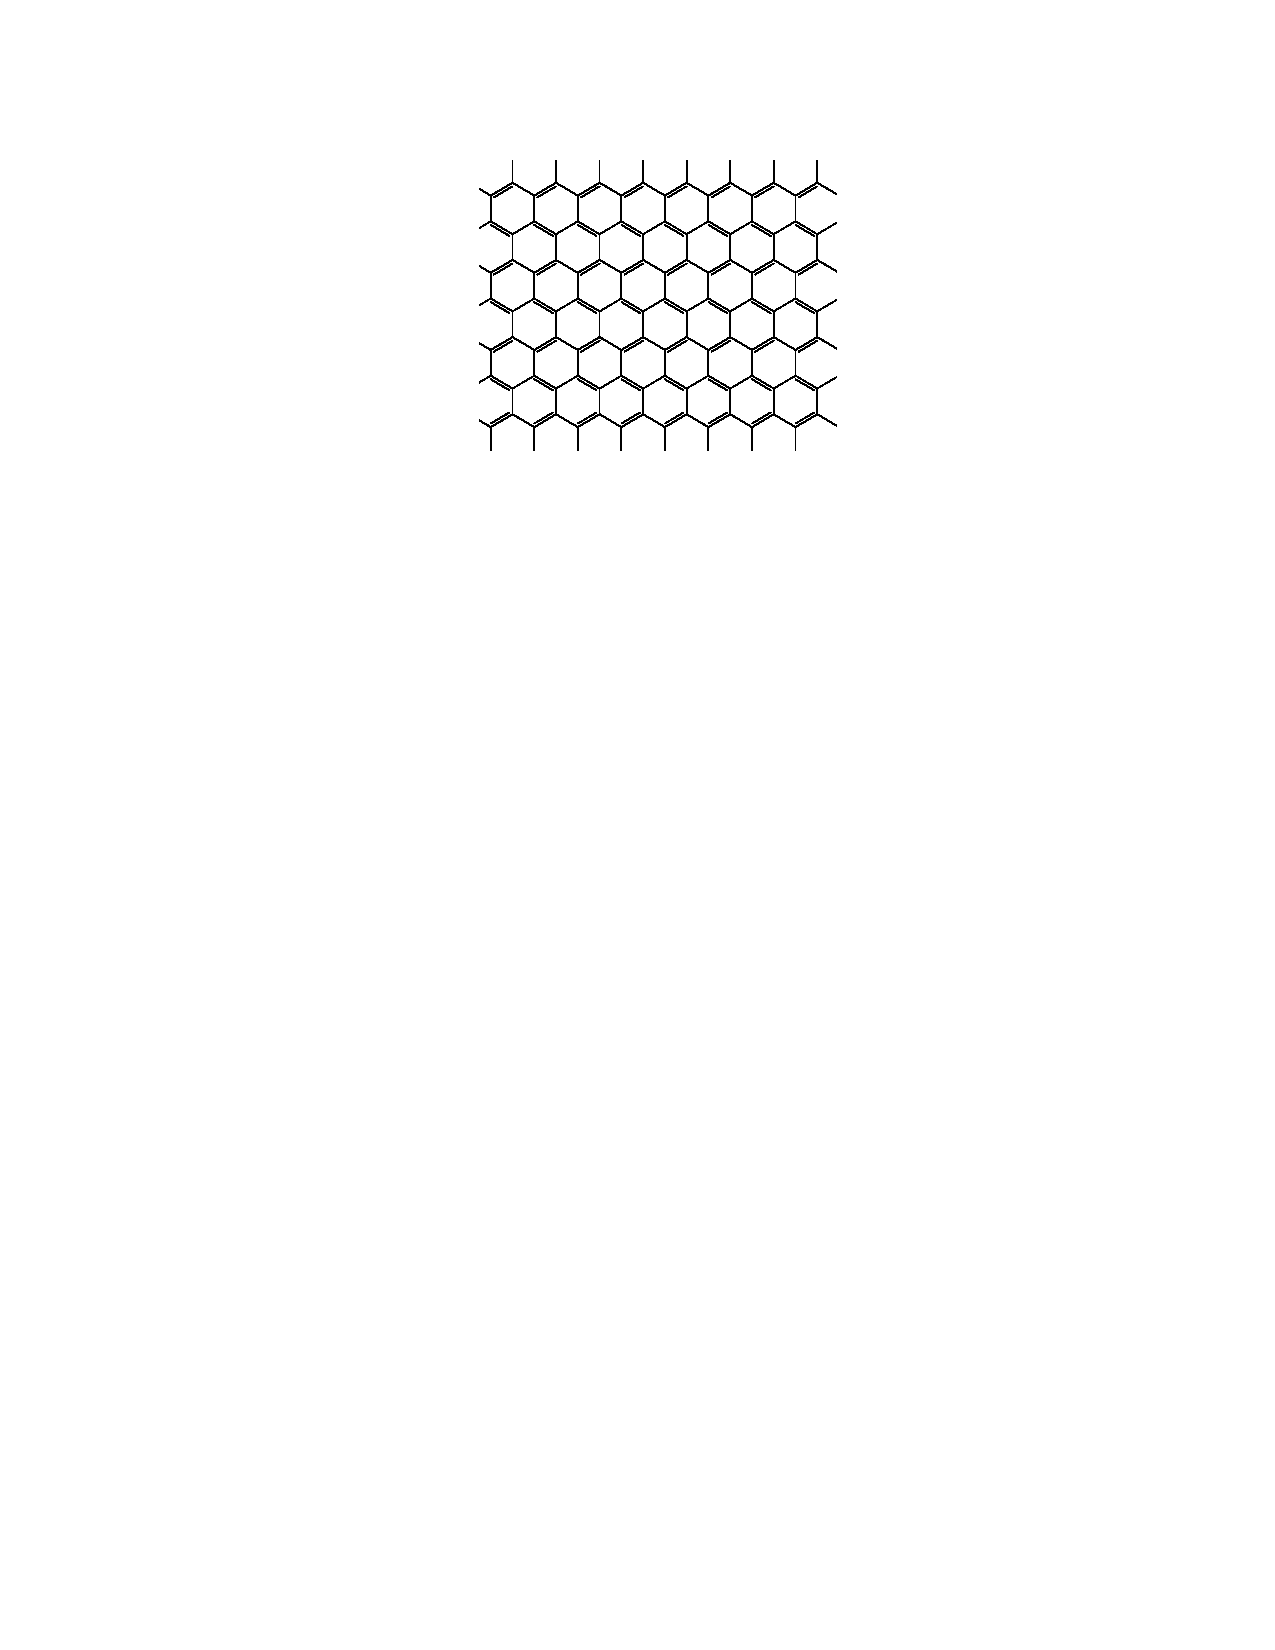
\includegraphics[width=7cm]{./pic/t18-1.pdf}
\end{figure}

对于一张$L_1=L_2=11\ \mathrm{\AA}$的正方形石墨烯片:

\noindent\textbf{18.4.}
6碳六边形单元中两个相邻碳之间的距离大约1.4 \AA。计算一张11 \AA $\times$ 11 \AA 的石墨烯片有多少个电子。在这个问题中你可以忽略边缘的电子(边长为$L$的正六边形的面积为$A=\frac{2\sqrt3}{2}L^2$)。

\noindent\textbf{18.5.} 计算HOMO的能量。

\noindent\textbf{18.6.} 计算LUMO的能量。

\noindent\textbf{18.7.}
LUMO和HOMO之间的能量差被称为带隙($E_g$)。计算带隙。

一维和二维势箱模型可以扩展到边长为$L_1$、$L_2$和$L_3$的三维长方体势箱中,从而得到下面的允许的能级的能量公式:

$$
E_{n_1,n_2,n_3}=\frac{h^2}{8m}\left(\frac{n^2_1}{L_1^2}+\frac{n^2_2}{L_2^2}+\frac{n^2_3}{L_3^2}\right)
$$

其中$n_1$、$n_2$和$n_3$分别是三个维度的量子数。对于一个边长为$L$的正方体势箱:

\noindent\textbf{18.8.} 给出5个能量不同且最低的能量表达式。

\noindent\textbf{18.9.} 画出展示了所有的五个能级的图,并指出每个能级的简并度。
